\chapter{Пластичность, остаточные напряжения и текстура}

\section{Диаграмма растяжения}

Растянем образец (рис.~\ref{fig:f7_ss}). Сначала напряжение растёт пропорционально деформации с наклоном $E$ ---
это упругость: снимите нагрузку, и образец вернётся к исходной длине. Выше \textbf{предела текучести}
$\sigma_y$ начинается пластическое течение. Деформация после разгрузки уже не исчезает: разгрузка идёт по
прямой с тем же наклоном $E$, и остаётся пластическая деформация $\eps_p$. Чтобы деформировать металл дальше,
нужно всё большее напряжение --- это \textbf{упрочнение}.

\begin{figure}[htbp]\centering
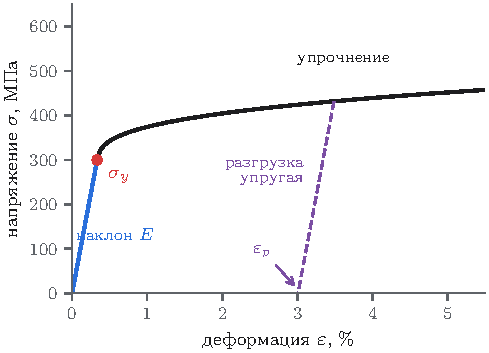
\includegraphics[width=0.6\linewidth]{f7_ss}
\caption{Схема диаграммы растяжения: упругий участок (наклон $E$), предел текучести $\sigma_y$, упрочнение;
разгрузка упругая, остаётся пластическая деформация $\eps_p$.}
\label{fig:f7_ss}
\end{figure}

Для оболочечных сплавов циркония при 300--400\degC{} предел текучести порядка 200--500~МПа: меньше у
рекристаллизованного металла, больше у холоднодеформированного и снятого от напряжений.

\section{Когда металл течёт при сложном нагружении}

В трубе напряжения не одноосные: под давлением окружное $\sigma_\theta$ вдвое больше осевого $\sigma_z$. Нужен
критерий текучести для любого напряжённого состояния. Гидростатическое давление на текучесть почти не влияет ---
дислокации двигает только касательное напряжение. Поэтому критерий строят по девиатору.
\begin{keyf}[Критерий Мизеса]
\[
\sigma_{\text{экв}} = \sqrt{\tfrac32\,s_{ij}s_{ij}}\;=\;\sigma_y
\]
(для плоского состояния $\sigma_1^2-\sigma_1\sigma_2+\sigma_2^2 = \sigma_y^2$).
\end{keyf}
Критерий Треска --- максимальное касательное напряжение $(\sigma_{\max}-\sigma_{\min})/2 = \sigma_y/2$. На плоскости
главных напряжений Мизес --- эллипс, Треска --- вписанный шестиугольник (рис.~\ref{fig:f7_yield}).

\begin{figure}[htbp]\centering
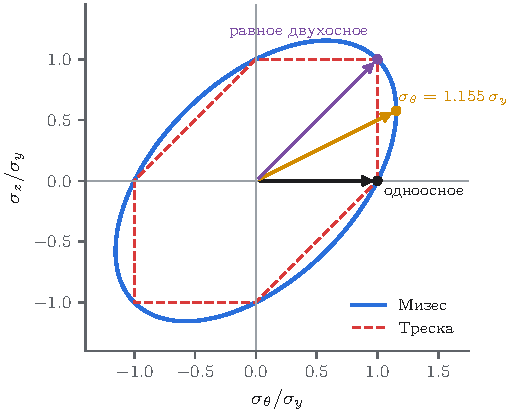
\includegraphics[width=0.52\linewidth]{f7_yield}
\caption{Поверхности текучести в плоскости $(\sigma_\theta,\sigma_z)$: Мизес (эллипс) и Треска (шестиугольник).
Стрелки --- пути нагружения: одноосное растяжение, труба с заглушками ($\sigma_z = \sigma_\theta/2$), равное
двухосное. Труба начинает течь при $\sigma_\theta\approx1.155\,\sigma_y$.}
\label{fig:f7_yield}
\end{figure}

\begin{idea}
Почему при $\sigma_z = \sigma_\theta/2$ труба выдерживает больше, чем стержень? Осевое растяжение уменьшает
девиатор: два растяжения частично «гасят» друг друга по сдвигу. Поэтому одинаковые окружные напряжения в
трубе и в кольце, растягиваемом в одном направлении, дают разную пластичность --- и разную переориентацию.
\end{idea}

\section{Дислокационная природа текучести}

Дислокация начинает скользить, когда касательное напряжение в её плоскости и направлении скольжения достигает
критического $\tau_c$. При одноосном растяжении это напряжение равно $\sigma\cos\varphi\cos\lambda$ (закон
Шмида; $\varphi$ и $\lambda$ --- углы нагрузки с нормалью к плоскости и с направлением скольжения). Упрочнение
возникает потому, что дислокации множатся и мешают друг другу: $\tau\approx\alpha\mu b\sqrt\rho$, где $\rho$ ---
плотность дислокаций (уравнение Тейлора).

В цирконии лёгкое скольжение одно --- призматическое $\{10\bar10\}\langle11\bar20\rangle$. Деформация вдоль оси $c$
требует пирамидального скольжения $\langle c+a\rangle$ (оно в несколько раз «твёрже») или двойникования. Поэтому
прочность зерна сильно зависит от того, как к нагрузке повёрнута ось $c$. Прочность трубы в целом зависит от
текстуры (раздел~\ref{sec:texture}). Анизотропную текучесть описывают критерием Хилла --- обобщением Мизеса с
разными весами для разных компонент напряжения.

\section{Пластическая аккомодация гидрида и память}

Упругие напряжения от гидрида --- порядка $\mu\eps^*\sim30~\text{ГПа}\cdot0.05\approx1.5$~ГПа. Это в несколько
раз выше предела текучести. Значит, вокруг всякого гидрида, кроме совсем мелкого, металл течёт. Оценим
размер пластической зоны для простейшей модели: жёсткий шар радиуса $a$ с линейным несоответствием $\delta$ в
идеально пластичной матрице (за зоной --- упругость, в зоне материал несжимаем). Объём, «выдавленный» шаром,
$4\pi a^3\delta$, должен равняться объёму, на который сдвигается упругая граница зоны радиуса $c$. Отсюда
\begin{keyf}[Пластическая зона вокруг включения]
\[
\Bigl(\frac{c}{a}\Bigr)^3 \approx \frac{6\mu\,\delta}{\sigma_y}.
\]
\end{keyf}
Для гидрида ($\mu = 33$~ГПа, $\delta\approx0.057$ --- треть объёмного несоответствия, $\sigma_y = 300$~МПа) зона в
3.4~раза больше самого гидрида (рис.~\ref{fig:f7_zone}). У настоящей пластинки зона вытянута вдоль неё и наиболее
сильна у торцов. Пластическое течение идёт рождением и выбросом дислокационных петель.

\fig{f7_zone}{а) Радиус пластической зоны вокруг несоразмерного включения в единицах его радиуса от предела
текучести матрицы при трёх несоответствиях. б) Схема: гидрид, пластический ореол и выброшенные дислокационные
петли.}

\begin{zrbox}
Пластическая аккомодация --- ключ к трём наблюдениям.
\begin{itemize}
\item \textbf{Гистерезис}: новый гидрид платит работой пластического течения, а при растворении эта работа не
  возвращается. Отсюда часть разрыва между TSSP и TSSD (глава~2).
\item \textbf{Память}: при растворении гидрида дислокации и остаточная деформация остаются. При следующем
  охлаждении гидрид выпадает там же --- места уже «подготовлены». Сколько памяти переживает выдержку при
  максимальной температуре, зависит от отжига (возврата) и проверяется опытами с многократными циклами.
\item \textbf{Коллективная пластичность}: когда гидридов много, их пластические зоны сливаются, и металл вокруг
  целой пачки пластинок течёт как одно целое. Это меняет поле напряжений, в котором зарождаются соседи.
\end{itemize}
\end{zrbox}

\section{Остаточные и межзёренные напряжения}

Даже без внешней нагрузки металл не свободен от напряжений. Их различают по масштабу:
\begin{itemize}
\item \textbf{I рода} --- на масштабе детали (после прокатки, сварки, изгиба);
\item \textbf{II рода} --- между зёрнами. В цирконии их создаёт анизотропия: при охлаждении зерно сжимается вдоль
  $c$ сильнее, чем поперёк, а соседи с другой ориентацией ему мешают. Оценка $\Delta\alpha\,\Delta T\,E$ даёт
  десятки МПа --- сопоставимо с нагрузками, при которых идёт переориентация;
\item \textbf{III рода} --- на масштабе дислокаций и включений (поле вокруг гидрида, глава~5).
\end{itemize}

\begin{zrbox}
Межзёренные напряжения разные в разных зёрнах, и каждое зерно «видит» внешнюю нагрузку со своей добавкой. Это
даёт разброс условий зарождения от зерна к зерну. Его величина --- один из параметров модели.
\end{zrbox}

\section{Текстура трубы}
\label{sec:texture}

Ориентации зёрен в трубе не случайны. Прокатка и отжиг выстраивают их так, что оси $c$ большинства зёрен лежат
в плоскости радиус--окружность и наклонены от радиального направления к окружному на $\pm(30$--$40)^\circ$. Это
\textbf{текстура}. Её изображают \textbf{полюсной фигурой}: стереографической проекцией, на которой отмечены
направления осей $c$ всех зёрен (рис.~\ref{fig:f7_texture}а).

Для гидридов удобна свёртка текстуры в три числа --- \textbf{факторы Кернса}:
\begin{keyf}[Факторы Кернса]
\[
f_d = \bigl\langle\cos^2\angle(\mathbf c,\mathbf d)\bigr\rangle_{\text{по объёму}},\qquad f_r+f_\theta+f_z = 1 .
\]
\end{keyf}
$f_r$ --- доля «ориентированности» осей $c$ по радиусу, $f_\theta$ --- по окружности, $f_z$ --- вдоль оси трубы. Для
типичных оболочек $f_r\approx0.5$--$0.7$, $f_\theta\approx0.25$--$0.35$, $f_z\approx0.05$--$0.1$.

\fig{f7_texture}{Схема текстуры трубы: оси $c$ наклонены от радиального направления к окружному на
$\pm35^\circ$ с разбросом $12^\circ$. а) Полюсная фигура (0002) в равноплощадной проекции, центр --- радиальное
направление. б) Факторы Кернса этого распределения.}

\begin{zrbox}
Теперь всё складывается. Гидрид ложится около базисной плоскости своего зерна (глава~5). В трубе с радиальной
текстурой базисные плоскости большинства зёрен лежат примерно вдоль окружности, поэтому без нагрузки гидриды
\emph{окружные}. Окружное напряжение облегчает выпадение в зёрнах, у которых ось $c$ ближе к окружному
направлению (глава~5): в них пластинка встаёт по радиусу. Таких зёрен немного --- им соответствует $f_\theta$.
Поэтому переориентация зависит от текстуры. Дополнительный путь дают межзёренные гидриды и цепочки
пластинок, переходящие из зерна в зерно.
\end{zrbox}

\section{Итог: из чего складывается переориентация}

Соберём главы вместе.
\begin{enumerate}
\item \textbf{Сколько выпадет и когда} --- линии растворимости TSSD и TSSP, гистерезис между ними (главы~1, 2).
\item \textbf{Где окажется водород} --- быстрая диффузия выравнивает концентрацию на масштабе зёрен. Водород
  стекается к растянутым местам: торцам пластинок, вершинам трещин (глава~3).
\item \textbf{Какой формы и в какой плоскости} --- тонкие пластинки около базиса: так меньше упругая энергия
  несоответствия (главы~4, 5).
\item \textbf{В каких зёрнах и когда зародится} --- барьер зарождения, в показатель которого входят упругая
  энергия, работа нагрузки, дефекты и границы (главы~5, 6).
\item \textbf{Как пластинки выстраиваются} --- поле соседей, пластическая аккомодация, память о прежних гидридах
  (главы~5, 7).
\item \textbf{Какая доля станет радиальной} --- конкуренция зёрен с разной ориентацией, то есть текстура (глава~7).
\end{enumerate}
Модель гидридов --- это численная реализация всех шести пунктов одновременно. Читать её код и учебник по ней
(\texttt{../textbook}) после этого фундамента должно быть заметно легче.

\begin{exercise}
Найдите окружное напряжение начала текучести трубы с заглушками по Мизесу и по Треска. Насколько они различаются?
\end{exercise}

\begin{exercise}
Выведите оценку размера пластической зоны $(c/a)^3 = 6\mu\delta/\sigma_y$. Для этого возьмите упругое решение
$u = B/r^2$ вне зоны, условие текучести на её границе и несжимаемость внутри.
\end{exercise}

\begin{exercise}
Оси $c$ всех зёрен лежат в плоскости радиус--окружность под углом $\pm\chi$ к радиусу. Найдите $f_r$ и $f_\theta$.
При каком $\chi$ они равны?
\end{exercise}
